\section{Motivating example}
\label{example}


%To have an overview of the challenge we work on, 
To illustrate the adressed challenge, let us have an example. 
Figure \ref{fig: BMM} shows an excerpt of the  version ~0.9.0 of "Modisco Discovery Benchmark" metamodel. %\footnote{\url{https://git.eclipse.org/r/plugins/gitiles/modisco/org.eclipse.modisco/+/refs/tags/0.12.1/org.eclipse.modisco.infra.discovery.benchmark/model/benchmark.ecore}}.
Modisco is an academic initiative project implemented in the Eclipse platform that has evolved numerous times in the past to support the development of model-driven tools, reverse engineering, verification, and transformation of existing software systems \cite{bruneliere2010modisco,bruneliere2014modisco}.
%consisting of 10 classes in the version of~0.9.0.
Figure \ref{fig: BMM} illustrates  some of the domain concepts \textbf{Discovery}, \textbf{Project}, and \textbf{ProjectDiscovery}  used for the discovery and reverse engineering of an existing software system. 
From these metaclasses, a first code API is generated, containing Java interfaces and their implementation classes, a factory, a package, etc. %(details of created files in table \ref{table: locationofMMelemen}). 
Listing \ref{lis:Modisco_Code_API_V1} shows a snippet of the generated Java interfaces and classes from the metamodel in Figure \ref{fig: BMM}. 

The generated code API is further enriched by the developers with additional code functionalities in the "Modisco Discovery Benchmark" project and its dependent projects as well.
For instance, by implementing the methods defined in metaclasses and advanced functionalities in new classes.
% (\eg language services, tooling, \dots).
Listing \ref{lis:Modisco_Code_External_V1} shows the two classes \texttt{Report} and \texttt{JavaBenchmarkDiscoverer} of the additional code ({\small\boxed{Line~4,8}} in the same project "Modisco Discovery Benchmark" and in another dependent project, namely the "Modisco Java Discoverer Benchmark" project).
%, namely the classes \texttt{CDOProjectDiscoveryImpl} and \texttt{JavaBenchmarkPackageImpl}. 
%
%One of the dependent projects on the Modisco discovery benchmark metamodel is Java Benchmark Discoverer. From this project, as an example, we select 3 classes shown in Listing \ref{lis:Modisco_Code_External_V1}. 
%
%In particular, the classes \texttt{CDOProjectDiscoveryImpl} and \texttt{JavaBenchmarkPackageImpl}, and \texttt{JavaDiscoveredProjectImpl}, which handles information and statistics about CDO and Java project. 
%
%the class \textit{CDOProjectDiscoveryImpl} gives information and statistics about CDO project Discovery. 
%Another dependent class \textit{JavaBenchmarkPackageImpl} that creates and initializes the package' methods %for Package models
%( or Benchmark models ? non). The last class is
%\textit{JavaDiscoveredProjectImpl} that contains different information and statistics about java discovered project. 
%The method \textit{initializePackageContents} (line 12) retrieves a \textit{ProjectDiscovery} instance to initialize the classes of the Java Benchmark Package. The method \textit{eBaseStructuralFeatureID} (line 24) returns the structural identifier of the feature relying on the type of its class.  
%
%From version 0.9.0 to 0.11.0, 
In version~0.11.0, the "Modisco Discovery Benchmark" metamodel evolved with several significant changes, among which the following impacting changes: \emph{1)} Renaming the property \texttt{DicoveryDate} of the class  \texttt{JavaBenchmarkDiscoverer} to \texttt{DiscoveryDate}, and \emph{2)} Moving the property \emph{discoveryTimeInSeconds} from metaclass \texttt{Discovery} to \texttt{DiscoveryIteration}.

%To analyze the consequences of the metamodel evolution on the additional code, we track the impacts of the following metamodel changes:
%\begin{enumerate}%[noitemsep,nolistsep]



    %\item Pulled the reference \textit{discoveries} from metaclass \texttt{DiscoveredProject} to \texttt{Benchmark}.
\begin{comment}
    

\begin{itemize}
    \item \emph{1)} Renaming the property \texttt{DicoveryDate} of the class  \texttt{JavaBenchmarkDiscoverer} to \texttt{DiscoveryDate}. % and \texttt{DiscoveredProject}.
    
   \item \emph{2)} Moving the property \emph{discoveryTimeInSeconds} from metaclass \texttt{Discovery} to \texttt{DiscoveryIteration}. 
\end{itemize} %\DK{maybe choose another rename and move ? averageSaveTimeInSeconds ?}
\end{comment}

\begin{figure}

\centering
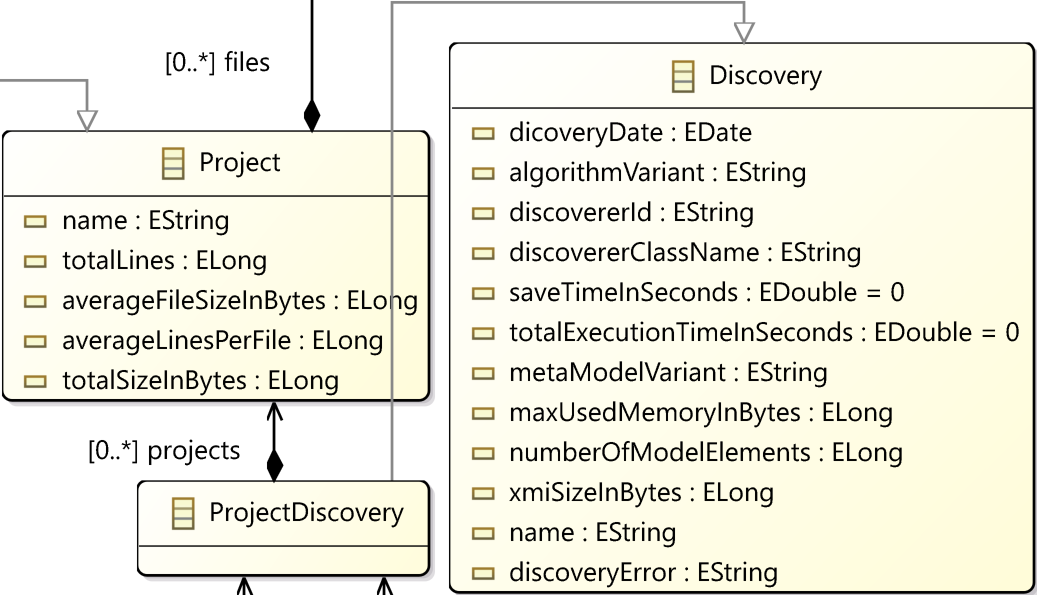
\includegraphics[width=0.45\textwidth]{pics/example.PNG}
\caption{Excerpt of Modisco Benchmark metamodel in version 0.9.0.}
\label{fig: BMM}
%\vspace{-5mm}
\end{figure}



After applying these modifications, the code of Listing \ref{lis:Modisco_Code_API_V1} is re-generated from the evolved version of the metamodel, which impacts the existing additional code depicted in Listings \ref{lis:Modisco_Code_External_V1}. 

\begin{lstlisting}[language=Java,breaklines=true,mathescape,literate={\-}{}{0\discretionary{-}{}{}},caption=Excerpt of the generated code in org.eclipse.modisco.infra.discovery.benchmark.,label={lis:Modisco_Code_API_V1}]
 //Discovery Interface
   public interface Discovery extends EObject {
  double getTotalExecutionTimeInSeconds();
  void setTotalExecutionTimeInSeconds(double value);
        ...
        }
 //Project Interface
   public interface ProjectDiscovery extends Discovery {...}
 //DiscoveryImpl Class
   public class DiscoveryImpl extends EObjectImpl implements Discovery {
     public double getTotalExecutionTimeInSeconds() {...}
     public void setTotalExecutionTimeInSeconds(double totalExecTime) {...}
         ...
    }
\end{lstlisting}
%xleftmargin=0.2cm,xrightmargin=0cm,framexleftmargin=+6pt,frame=single,
\begin{lstlisting}[language=Java,breaklines=true,mathescape,literate={\-}{}{0\discretionary{-}{}{}},caption=Excerpt of the additional code V1.,label={lis:Modisco_Code_External_V1}]
  
   public class Report {
    ...
       discovery.(*\ul{setDiscoveryTimeInSeconds}*)(...);
   }
    
   public class JavaBenchmarkDiscoverer extends AbstractModelDiscoverer<IFile> {
    ...
       discovery.(*\ul{setDicoveryDate}*)(new Date());
    ...
   } 
\end{lstlisting}


%%%%%%%%%%%%%%%%%%%%%%%%%%%%%%%%%%%%%%%%%%%%%%%%%%%%%%%%%%%
%%                   Now the evolved code                %%
%%%%%%%%%%%%%%%%%%%%%%%%%%%%%%%%%%%%%%%%%%%%%%%%%%%%%%%%%%%
\setulcolor{green} 
%\setstcolor{green}
%\setstcolor{green}
%,xleftmargin=0.2cm,,xrightmargin=-0cm,framexleftmargin=+6pt,frame=single
\begin{lstlisting}[language=Java,breaklines=true,mathescape,literate={\-}{}{0\discretionary{-}{}{}},caption=Excerpt of the additional code V2.,label={lis:Modisco_Code_External_V2}]
  
   public class Report {
    ...
       discovery.(*\ul{getIterations().get(0).}*) 
                    (*\ul{setDiscoveryTimeInSeconds}*)(...);
    ...
   }
   
   public class JavaBenchmarkDiscoverer extends AbstractModelDiscoverer<IFile> {
    ...
       discovery.(*\ul{setDiscoveryDate}*)(new Date());
    ...
   }
\end{lstlisting}




The resulting errors in the original code in version 0.9.0 are underlined in red in Listing \ref{lis:Modisco_Code_External_V1}. Listing \ref{lis:Modisco_Code_External_V2} presents the final result of the manual developer's co-evolution in version 0.11.0. The co-evolved code is underlined in green. 
% Expected co-evolution ?
The changes \textit{rename} of the property \textit{ DicoveryDate} and the \textit{move} of the property \emph{discoveryTimeInSeconds} impact their usages ({\small\boxed{Line~4,8}} in Listing~\ref{lis:Modisco_Code_External_V1}). The impact of renaming \textit{ DicoveryDate} is co-evolved by replacing \textit{setDicoveryDate} by \textit{setDiscoveryDate}. The impact of moving the property \emph{discoveryTimeInSeconds} is co-evolved by extending the call path of the method \emph{setDiscoveryTimeInSeconds} through the reference \textit{iterations} by calling the method \textit{getIterations} and getting the first element of the returned list of DiscoveryIteration objects.

%The above examples show the importance of correctly matching the different code usages of the generated code with the metamodel evolution changes to co-evolve them with the appropriate resolutions.  
Developers unfortunately manually co-evolve the code, which is tedious, error-prone, and time-consuming. 
One help developers get is from the IDE and the provided quick fixes. For example, when using Eclipse quick fixes to co-evolve these errors, it suggests creating the method \texttt{setDiscoveryTimeInSeconds} in the class \texttt{Discovery}, which does not meet the required co-evolutions shown in Listing~\ref{lis:Modisco_Code_External_V2}.

With the ever-growing popularity and promising results of LLMs, a developer can prompt an LLM to suggest a co-evolution. 
For example, 
%To motivate more our work, 
we asked ChatGPT to co-evolve the error resulted from moving the property \emph{discoveryTimeInSeconds} by giving the erroneous code ({\small\boxed{Line~4}} in Listing~\ref{lis:Modisco_Code_External_V1})  with the message of the error taken from eclipse Problems window. This is the first intuition when using ChatGPT because the developer does not know necessarily the metamodel change causing the error and finding it due to the abstraction gap is a tedious and error-prone task. Figure \ref{fig: chatgptanswer} shows that ChatGPT proposes to create a method named \emph{setDiscoveryTimeInSeconds} in the class \emph{Discovery}, which is totally wrong because it does not fit the causing change. 

Our Hypothesis is that the LLM fails because our problem is more complex than simply repairing a code error. It must understand the original impacting metamodel change traced to the code error, as well as the abstraction gap between the two artefacts of metamodels and code. After improving the prompt, \LLM succeeded to give the right resolution as show in Figure \ref{fig: chatgptimprovedanswer}.
Our vision is that this contextual rich information must be injected in the prompt.
Thus, the quality of the prompt is a key for the LLM to solve this problem of metamodels and code co-evolution. %Indeed, it is a hard problem due to the abstraction gap between the two artefacts of metamodels and code. This context should be part of the prompt as well as the impacting metamodle change that must be traced to the code error. 

%by giving only the errouneous ({\small\boxed{Line~4}} in Listing~\ref{lis:Modisco_Code_External_V1}). Chatgpt answer in this case was totaly wrong. Thus, we injected the change information in the request and asked Chatgpt to coevolve the same error. Figure \ref{fig: chatgptanswer} shows that even adding the change information did not help chatgpt to find the right resolution.
%
The next section presents our contribution for a contextualized information rich prompts-based co-evolution of metamodel and code using LLMs.  


\begin{figure}[t]
\centering
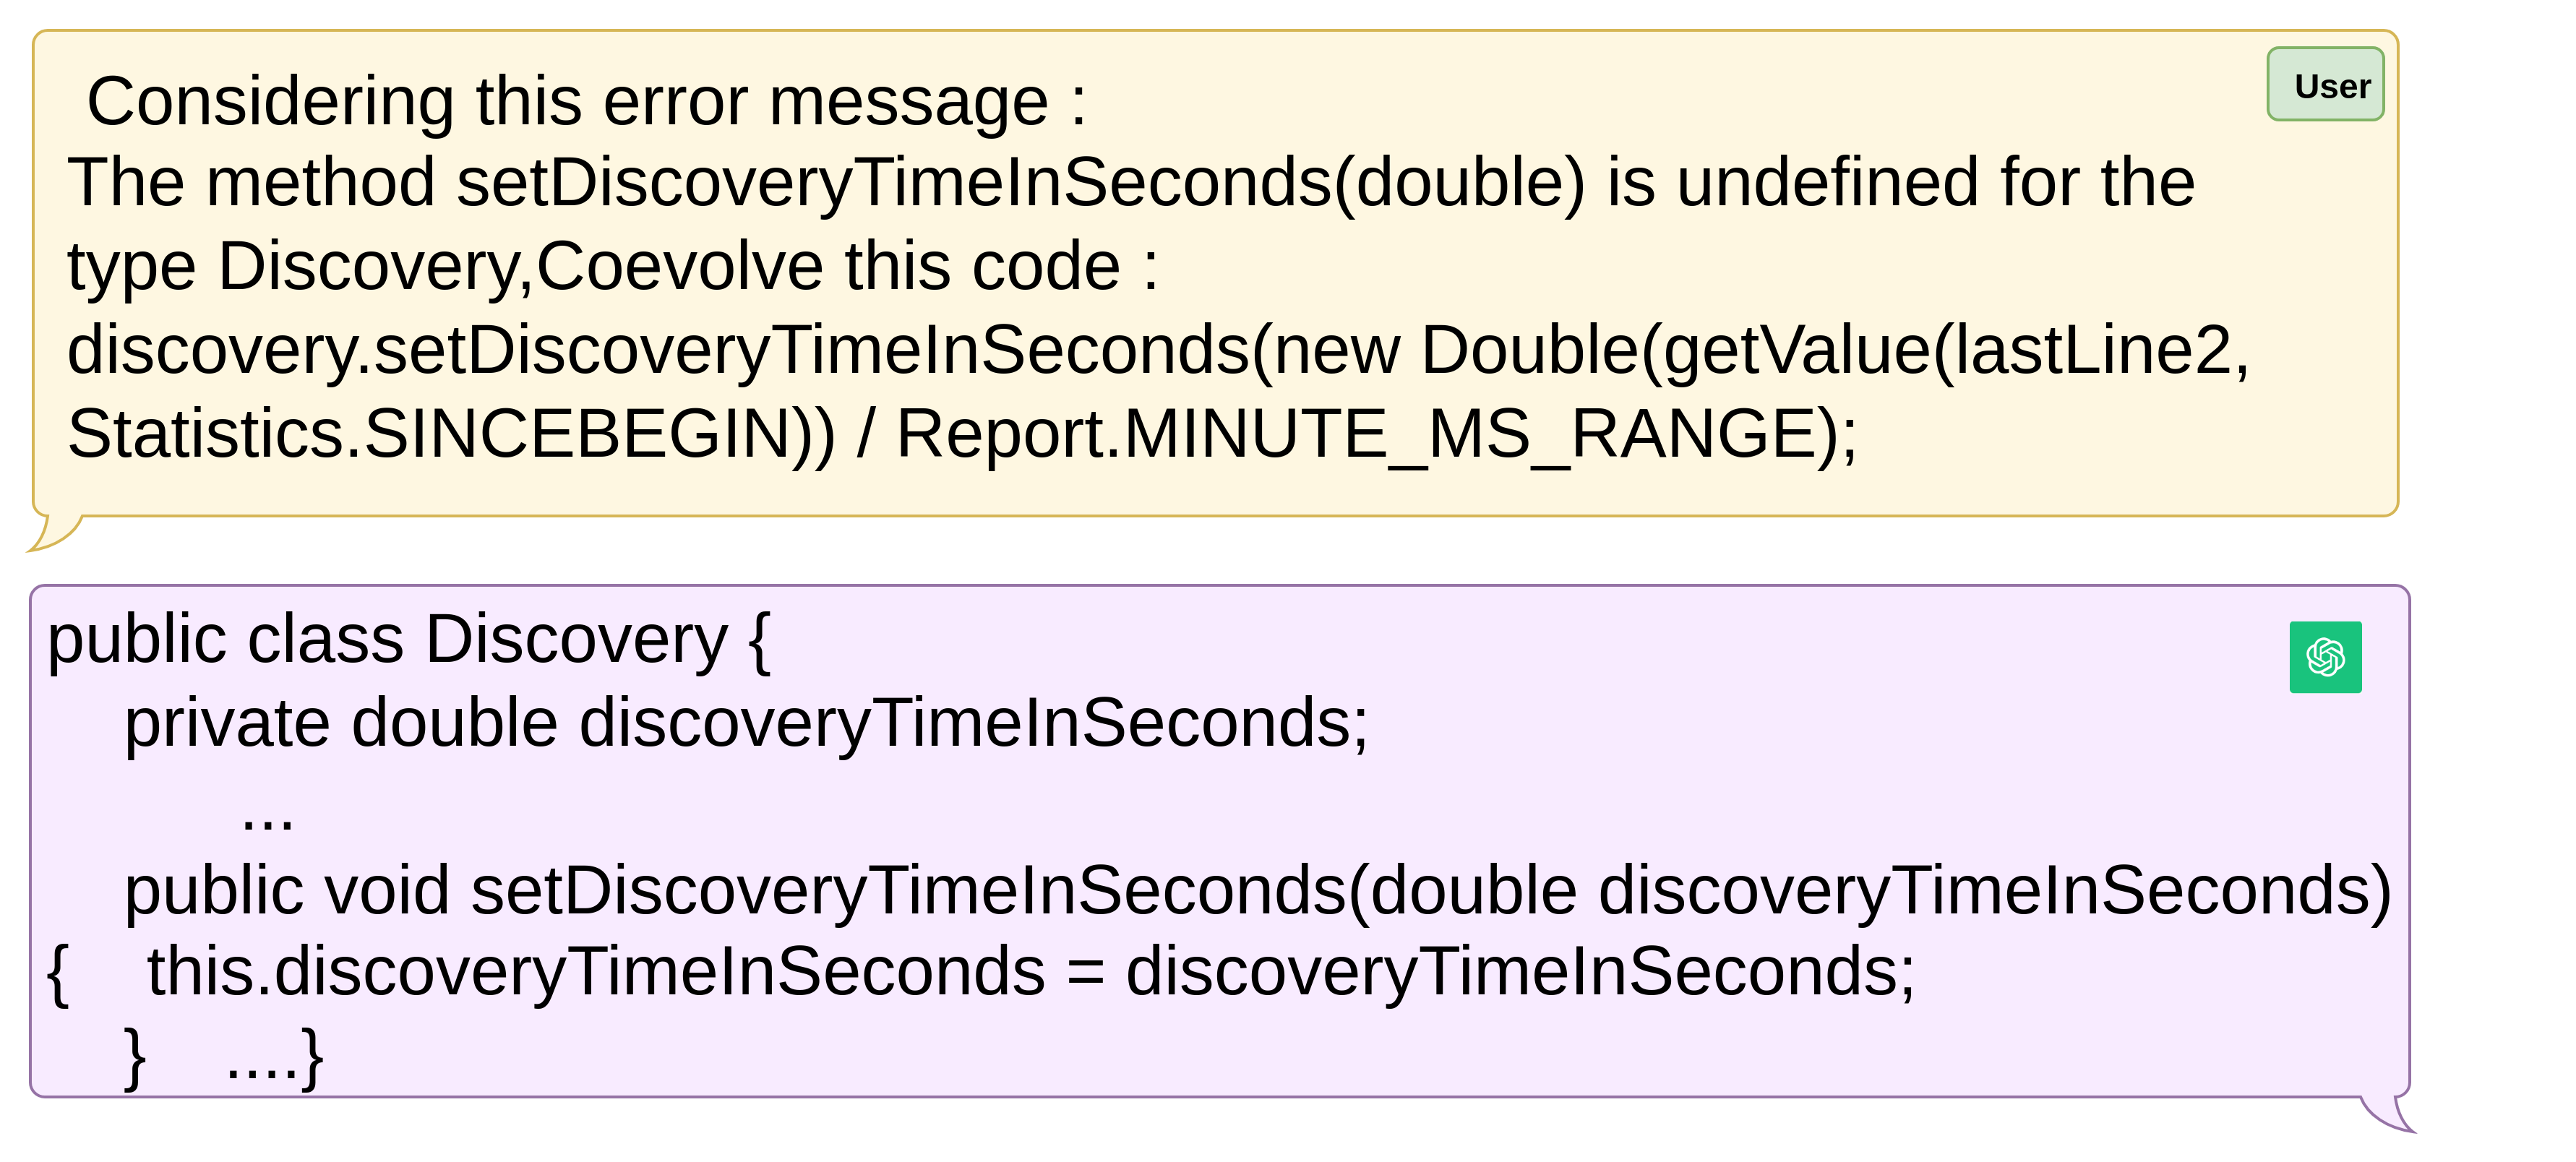
\includegraphics[width=0.48\textwidth]{pics/chatgptprimitiveanswer.png}
\caption{ChatGPT primitive answer to the naive prompt.}
\label{fig: chatgptanswer}
%\vspace{-5mm}
\end{figure}

\begin{figure}[t]
\centering
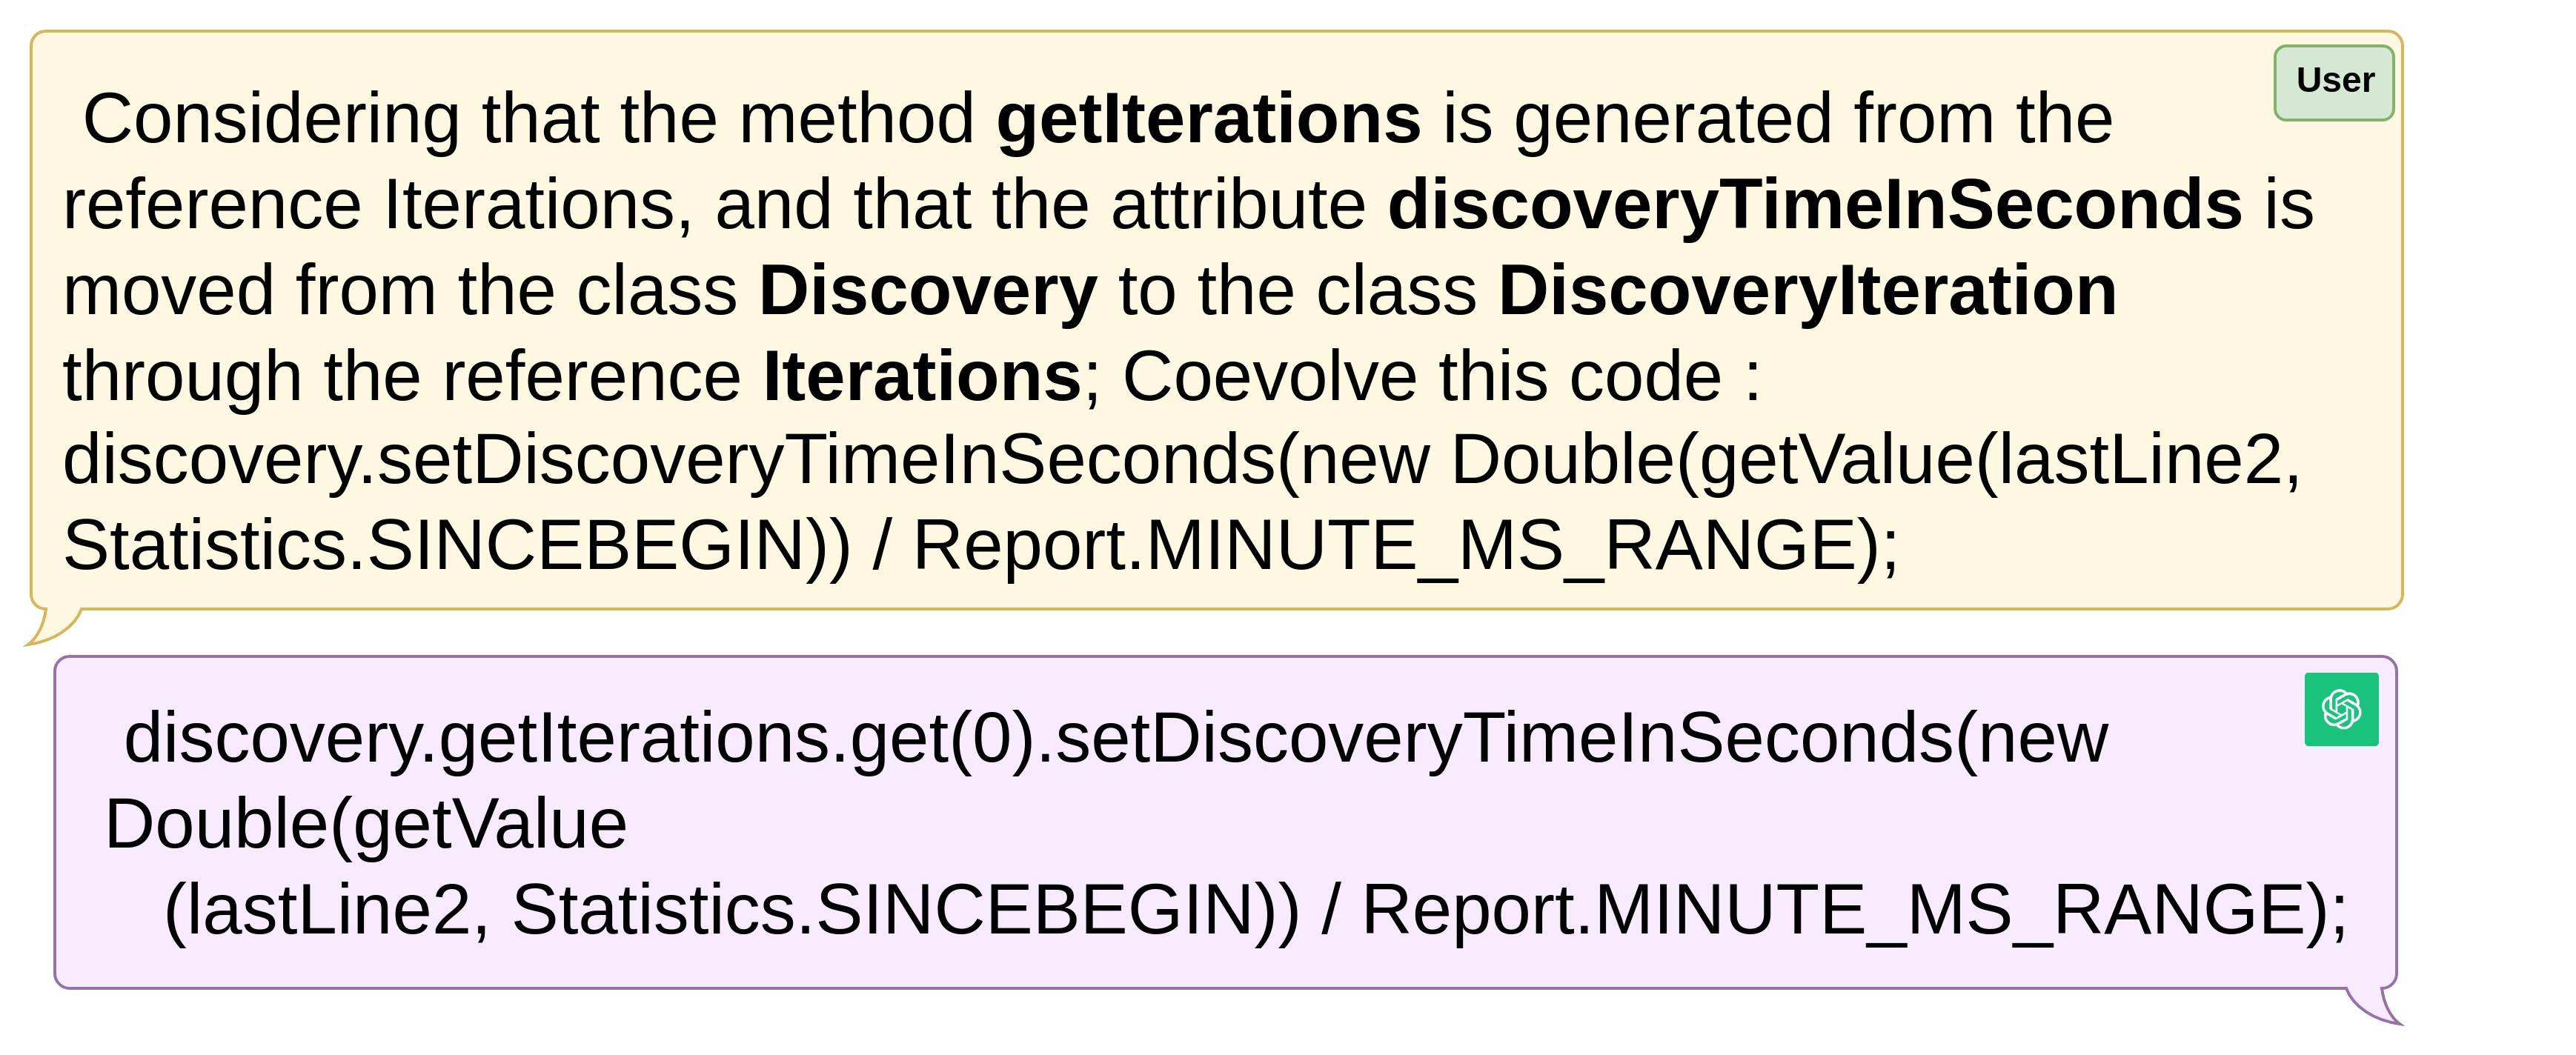
\includegraphics[width=0.48\textwidth]{pics/chatgptimprivedanswer.png}
\caption{\LLM improved answer with the enriched prompt with contextual information.}
\label{fig: chatgptimprovedanswer}
\vspace{-5mm}
\end{figure}